\chapter{Number Theory}

To understand the internals SNARKs it is foremost important to understand the basics of finite field arithmetics AND STUFF.

%Summary of this chapter
We therefore start with a brief introduction to fundamental algebraic terms like fields, field extensions AND STUFF . We define these terms in the general abstract way of mathematics, hoping that the non mathematical trained reader will gradually learn to become comfortable with this style. We then give basic examples, that likely all of us know and do basic computations with these examples. 

The motivated reader is then encuraged to do some exercises from  the apendix of this chapter.

\section{Preliminaries}
INTO-BLA

When you read papers about cryptography or mathematical papers in general, you will frequently stumble across terms like \textit{fields}, \textit{groups},\textit{rings} and similar. As we will use these terms repeatedly, we have to start this chapter with a short introduction to those terms.

In a nutshell, those terms define sets that are in some sense analog to numbers, in that you can add, subtract, multiply or divide. Or more abstractly those sets have certain ways to combine two elements into a new element.

We know many example like the natural numbers, the integers, the ratinal or the real numbers from school and they are in some sense already the most fundamental examples

Lets start with the concept of a group. Remember back in school when we learned about addition and subtraction of integers. We learned that we can always add to integers and that the result is an integer again. We also learned that nothing happens, when we add zero to any integer, that it doesn't matter in which order we add a given set of integers and that for every integer there is always a negative counterpart and if we add both together we get zero. 

Distilling these rules to the smallest list of properties and make rthem abstract we arrive at the definition of a group:
\begin{definition}[Group]
A grou $ (\G, \cdot) $ is a set $ \G$, together with a map $ \cdot: \G \cdot \G \to \G $, called the group law (or \textit{addition} respectively \textit{multiplication}), such that the following hold:
\begin{itemize}
\item (Existence of a neutral element) There is a $e\in\G$ for all $g\in\G$, such that $e\cdot g=g$ as well as $g\cdot e = g$.
\item (Existence of an inverse) For every $g\in\G$ there is a $g^{-1}\in\G$, such that $g\cdot g^{-1}=e$ as well as $g^{-1}\cdot g = e$.
\item (Associativity) For every $g_1,g_2,g_3\in\G$ the equation 
$g_1\cdot(g_2\cdot g_3) = (g_1\cdot g_2)\cdot g_3$ holds.
\end{itemize}
In addition a group is called commutative if the equation 
$g_1\cdot g_2 = g_2 \cdot g_1$ holds for all $g_1,g_2\in\G$.

A group is called finite, if the underlying set of elements is finite.

An element $g\in G$ is called a \textbf{generator} of that group if every other group element can be generated by combining $g$ with itself only.
\end{definition}
\begin{remark}
By definition, a generator is a special element, that can generate the entire group, by adding it repeatedly to itself. For example the number $1$ is a generator for the natural numbers (not a group), as you can compute any natural number by adding 1 repeatedly to itself.  
\end{remark}
\begin{remark}
If not stated otherwise, we will use the $+$ symbol for the group law of a commutative group. In that case we use the symbol $0$ for the neutral element and write the inverse as $-x$.
\end{remark}
% https://doc.sagemath.org/html/en/reference/categories/sage/categories/groups.html
Sagemath comes with a definition of the category of all groups, which inherits the properties of \textit{Magmas}, which are like groups but without the notion of inverses. For our purposes we only need commutative groups and in particular finite and cyclic groups.

\begin{sagecommandline}
sage: Groups()
sage: CommutativeAdditiveGroups()
sage: FiniteGroups()
\end{sagecommandline}

\begin{example}[Integer Addition and Subtraction]
As previously described, the set of integers together with integer addition is the archetypical example of a group. In contrast to our definition above the group laws is usually not written as $\cdot$, but as $+$ instead. The neutral element is the number $0$ and the inverse of a natural number $x\in\Z$ is the negative $-x$. Since $x+y=y+x$ this is an example of a commutative group.
\end{example}
\begin{example}[The trivial group]
The most basic example of a group, is group with just one element $\{\bullet\}$ and the group law $0\cdot 0=0$. This group can be defined in many ways. In sage it is defined as the group of all permutations of a single element (which is just the identity permutation that is doing nothing). Therefor in sage we can write
 \begin{sagecommandline}
sage: TrivialGroup = SymmetricGroup(1)
\end{sagecommandline}
\end{example}
Now thinking of integers again, we know, that there are actually two operations addition and multiplication, such that that they interact in a certain way. This is captured by the concept of a ring, where integers are the most basic example in a sense



\begin{definition}[Commutative Ring with Unit]
A ring $ (R, +, \cdot) $ is a set $R$, provided with two maps $ +: R \cdot R \to R $ and $ \cdot: R \cdot R \to R $, called \textit{addition} and \textit{multiplication}, such that the following conditions hold:
\begin{itemize}
\item $ \left (R, + \right) $ is a commutative group, where the neutral element is denoted here with $ 0 $.
\item (Existence of a unit) There is an element $1\in R$ for all $g\in R$, 
\item (Associativity) For every $g_1,g_2,g_3\in\G$ the equation 
$g_1\cdot(g_2\cdot g_3) = (g_1\cdot g_2)\cdot g_3$ holds. 
\item (Distributivity) For all $ g_1, g_2, g_3 \in R $ the distributive laws apply:
$$ g_1 \cdot \left (g_2 + g_3 \right) = g_1 \cdot g_2 + g_1 \cdot g_3 \quad \text{and} \quad
\left (g_1 + g_2 \right) \cdot g_3 = g_1 \cdot g_3 + g_2 \cdot g_3 $$
\item COMMUTATIVITY
\end{itemize}
\end{definition}

\begin{sagecommandline}
sage: CommutativeRings()
sage: CommutativeRings().super_categories()
\end{sagecommandline}

\begin{example}[The Ring of Integers] The set $\Z$ of integers with the usual addition and multiplication is a ring. In sage the ring of integers is called as follows and as we know, not all elements have multiplicative inverses
\begin{sagecommandline}
sage: ZZ # A sage notation for the Ring of integers
sage: ZZ(5) # Get an element from the Ring of integers
sage: ZZ(5) + ZZ(3)
sage: ZZ(5) * ZZ(3)
sage: ZZ.random_element(10**50)
sage: ZZ(27713).str(2) # Binary string representation
sage: ZZ(27713).str(16) # Hexadecimal string representation
\end{sagecommandline}
\end{example}
\begin{example}[Underlying additive group of a ring] Every ring $(R,+,\cdot)$ gives rise to group, if we just forget about the multiplication
\end{example}
The following example is more interesting, as it introduces the concept of so called addition and multiplication table. To understand those tables BLA....
\begin{example} Let $S:=\{\bullet,\star,\odot,\otimes\}$ be a set that contains four elements and let adiition and multiplication on $S$ be defined as follows:
\begin{center}
  \begin{tabular}{c | c c c c c c}
    $\cup$ & $\bullet$ & $\star$ & $\odot$ & $\otimes$ \\\hline
    $\bullet$ & $\bullet$ & $\star$ & $\odot$ & $\otimes$ \\
    $\star$ & $\star$ & $\odot$ & $\otimes$ & $\bullet$ \\
    $\odot$ & $\odot$ & $\otimes$ & $\bullet$ & $\star$ \\
    $\otimes$ & $\otimes$ & $\bullet$ & $\star$ & $\odot$ \\
  \end{tabular} \quad \quad \quad \quad
  \begin{tabular}{c | c c c c c c}
$ \circ $ & $\bullet$ & $\star$ & $\odot$ & $\otimes$ & \\\hline
        $\bullet$ & $\bullet$ & $\bullet$ & $\bullet$ & $\bullet$ &\\
        $\star$ & $\bullet$ & $\star$ & $\odot$ & $\otimes$ &\\
        $\odot$ & $\bullet$ & $\odot$ & $\bullet$ & $\odot$ &\\
        $\otimes$ & $\bullet$ & $\otimes$ & $\odot$ & $\star$ &\\
  \end{tabular}
\end{center}
Then $(S,\cup,\circ)$ is a ring with unit $\star$ and zero $\bullet$. It therefore makes sense to ask for solutions to equations like this one:
Find $x\in S$ such that
$$
\otimes \circ (x \cup \odot ) = \star
$$
To see how such an "alien equation" can be solved, we have to keep in mind, that rings behaves mostly like normal number when it comes to bracketing and computation rules. The only differences are the symbols and the actual way to add and multiply. With this we solve the equation for $x$ in the "usual way"
\begin{align*}
\otimes \circ (x \cup \odot ) &= \star & \text{distributive law}\\
\otimes \circ x \cup \otimes \circ \odot  &= \star & \otimes \circ \odot = \odot\\
\otimes \circ x \cup \odot  &= \star & \text{add the additive inverse to both sides}\\
\otimes \circ x \cup \odot \cup -\odot  &= \star \cup -\odot\\
\otimes \circ x \cup \bullet &= \star \cup -\odot & \text{inverse property}\\
\otimes \circ x &= \star \cup -\odot & \text{neutral element can be deleted} \\
\otimes \circ x &= \star \cup \odot & -\odot = \odot \text{from addition table} \\
\otimes \circ x &= \otimes  & \star \cup \odot = \otimes \text{from addition table}\\
(\otimes)^{-1}\circ \otimes \circ x &= (\otimes)^{-1}\circ \otimes & \text{multiply with the multiplicative inverse}\\
\otimes\circ \otimes \circ x &= \otimes\circ \otimes\\
\star \circ x &= \star\\
x &= \star
\end{align*}
On the other hand, EQUATION $2x=3$ has no sultion and equation BLA has more then one solution. So rings are sometimes different from numbers. When we want more we need fields .... BLAHHHH EXPAND
\end{example}
It is a good and fundamental exercise in mathematics to understand examples like this in detail as it helps the reader to loosen the connection to what "should be" numbers and what not.


\begin{definition}[Field]
A field $ (\F, +, \cdot) $ is a set $ \F$, provided with two maps $ +: \F \cdot \F \to \F $ and $ \cdot: \F \cdot \F \to \F $, called \textit{addition} and \textit{multiplication}, such that the following conditions holds
\begin{itemize}
\item $ \left (\F, + \right) $ is a commutative group, where the neutral element is denoted by $ 0 $.
\item $ \left (\F \setminus \left \{0 \right \}, \cdot \right) $ is a commutative group, where the neutral element is denoted by $ 1 $.
\item (Distributivity) For all $ g_1, g_2, g_3 \in \F $ the distributive laws apply:
$$ g_1 \cdot \left (g_2 + g_3 \right) = g_1 \cdot g_2 + g_1 \cdot g_3 \quad \text{and} \quad
\left (g_1 + g_2 \right) \cdot g_3 = g_1 \cdot g_3 + g_2 \cdot g_3 $$
\end{itemize}
The \textit{characteristic} of a field $ \F $ is the smallest natural number $ n \geq 1 $, for which the $ n $ -fold sum of $ 1 $ equals zero, i.e. for which $ \sum_{i = 1} ^ n 1 = 0 $.

If such a $ n> 0 $ exists, the field is also called of \textit{finite characteristic}. If, on the other hand, every finite sum of $1$ is not equal to zero, then the field is defined to have characteristic $ 0 $.
\end{definition}
So a field is a commutative ring with unit, such that every element other the the neutral element of addition has an inverse.

\begin{sagecommandline}
sage: Fields()
\end{sagecommandline}

\begin{example}[Field of rational numbers] Probably the best known example of a field is the set of rational numbers $\mathbb{Q}$ together with the usual definition of addition, subtraction, multiplication and division. In sage rational numbers are called like this
\begin{sagecommandline}
sage: QQ
sage: QQ(1/5) # Get an element from the field of rational numbers
sage: QQ(1/5) / QQ(3) # Division
\end{sagecommandline}
\end{example}
\begin{example}[Field with two elements] It can be shown that in any field, the neutral element $0$ of addition must be different from the neutral element $1$ of multiplication, that is we always have $0\neq 1$ in a field. From this follows that the smallest field must contain at least two elements and as the following addition and multiplication tables show, there is indeed a field with two elements, which is usually called $\F_2$:

Let $\F_2:=\{0,1 \}$ be a set that contains two elements and let addition and multiplication on $\F_2$ be defined as follows:
\begin{center}
  \begin{tabular}{c | c c c}
    + & 0 & 1 \\\hline
    0 & 0 & 1\\
    1 & 1 & 0 \\
  \end{tabular} \quad \quad \quad \quad
  \begin{tabular}{c | c c c}
$\cdot$ & 0 & 1 \\\hline
      0 & 0 & 0 \\
      1 & 0 & 1 \\
  \end{tabular}
\end{center}
For reasons we will understand better in XXX, sage defines this field as a so called Galois field with 2 elements. It is called like this:
\begin{sagecommandline}
sage: GF(2)
sage: GF(2)(1) # Get an element from GF(2)
sage: GF(2)(1) + GF(2)(1) # Addition
sage: GF(2)(1) / GF(2)(1) # Division
\end{sagecommandline}
\end{example}


\subsection{Integer Arithmetics}
\label{integer_arithmetics}
We start by a recapitulation of basic arithmetics as most of us will probably recall from school.

As we have seen in the previous section integers form a ring and division is not well defined. However one of the most basic but at the same time highly important technique, that every reader must become familiar with is the following (kind of) replacement for devision of integers called \textit{Euklidean division} (\cite{AL}
\begin{theorem}[Euklidean Division]
Let $ a \in \Z $ be an integer and $ b \in \N $ a natural number. Then there are always two numbers $ m \in \Z $ and $ r \in \N $, with $ 0 \leq r <b $ such that
\begin{equation}
\label{eq: euklidean_division}
a = m \cdot b + r
\end{equation}
This decomposition of $a$ given $b$ is called \textbf{Euklidean division} or \textbf{division with remainder} and $ a $ is called the \textbf{divident}, $ b $ is called the \textbf{divisor},$m$ is called the quotient and $r$ is called the \textbf{remainder}. 
\end{theorem}
\begin{remark}
\label{eq: euklidean_division_notation}
If $ a, b, m $ and $ r $ satisfy the equation (\ref{eq: euklidean_division}), we often write $ \Zdiv{a}{b}: = m $ to describe the quotient and use the symbol $ \Zmod{a}{b}: = r $ for the remainder. We also say, that an integer $ a $ is divided by a number $ b $ if $ \Zmod{a}{b} = 0 $ holds. In this case we also write $ a | b $ (\cite{AL} Note 1 below).
\end{remark}
\begin{example}
Using our previously defined notation, we have $ \Zdiv{-17}{4 } = - 5 $ and $ \Zmod{-17}{4} = 3 $, because $ -17 = -5 \cdot 4 + 3 $  is the Euklidean division of $-17$ and $4$ (Since the remainder is by definition a non-negative number). In this case $4$ does not divide $-17$ as the reminder is not zero. Writing $-17 | 4$ therefore has no meaning.

On the other hand we can write $12 | 4$, since $4$ divides $12$, as $ \Zmod{12}{4} = 0 $.

\begin{sagecommandline}
sage: ZZ(-17) // ZZ(4) # Integer quotient 
sage: ZZ(-17) % ZZ(4) # remainder 
sage: ZZ(-17).divides(ZZ(4))
sage: ZZ(4).divides(ZZ(12))
\end{sagecommandline}
\end{example}
A fundamental property of Euclidean division is that both the quotient and the remainder exist and are unique. The result is therefore independent of any algorithm that actually does the computation.

Methods for computing the division with remainder are called \textit{integer division algorithms}. Probably the best known algorithm is the so called \textit{long division}, that most of us might have learned in school. It should be noted however that there are faster algorithms like \textit{Newton–Raphson division} known.

As long division is the standard algorithm used for pen-and-paper division of multi-digit numbers expressed in decimal notation, the reader should become familiar with this algorithm as we use it all over this book when we do simple pen-and-paper computations.

In a nutshell, the algorithm shifts gradually from the left to the right end of the dividend, subtracting the largest possible multiple of the divisor (at the digit level) at each stage; the multiples then become the digits of the quotient, and the final difference is then the remainder. To be more precise one version of the algorithm looks like this:

\begin{algorithmic}
\State Divide $n$ by $d$
\State If $d = 0$ then error(DivisionByZeroException) end
\State $Q \leftarrow 0 $ -- Initialize quotient to zero
\State $R \leftarrow 0 $ -- Initialize remainder to zero               
\State TO APPEAR
\end{algorithmic}

\begin{example}[Integer Log Division] To give an example of the basic integer long division algorithm most of us learned at school, lets divide the integer $157843853$ by the number $261$. 

So the goal is to find quotient and reminder $m,r \in \N$ such that
$$157843853 = 261 * m +r$$
holds. Using a notation that is mostly used in Commonwealth countries we can then compute
%\longdivision{157843853}{261} 

TO-APPEAR 
\end{example}

\begin{sagecommandline}
sage: ZZ(157843853).quo_rem(ZZ(261)) # Euclidean Division
sage: ZZ(604765)*ZZ(261) + ZZ(188) # check
\end{sagecommandline}


Another important algorithm frequently used in computations with integers is the so-called \textit{extended Euclidean algorithm}, which calculates the greatest common divisor $ gcd (a, b) $ of two natural numbers $ a $ and $ b \in \N $, as well as two additional integers $ s, t \in \Z $, such that the equation
\begin{equation}
\label{eq: erw_Eukl_algo}
gcd (a, b) = s \cdot a + t \cdot b
\end{equation}
holds. Two numbers are called \textbf{relative prime}, if their greates common divisor is $1$.

The following pseudocode shows in detail how to calculate these numbers with the extended Euclidean algorithm (\cite{JB} chapter 2.9):




\begin{definition}
\label{theorem: ext_Euclid}
Let the natural numbers $ a, b \in \N $ be given. Then the so-called \textit{extended Euclidean algorithm} is given by the following calculation rule:
\begin{algorithmic}
\State $ \begin{array}{ccccc}
r_0: = a, & r_1: = b, & s_0: = 1, & s_1: = 0, & k: = 1
\end{array} $
\While{$ r_{k} \neq 0 $}
\State $ q_k: = \Zdiv{r_{k-1}}{r_k} $
\State $ r_{k + 1}: = r_{k-1} -q_k \cdot r_k $
\State $ s_{k + 1}: = s_{k-1} -q_k \cdot s_k $
\State $ k \gets k + 1 $
\EndWhile
\end{algorithmic}
As a result, the algorithm computes the integers $ gcd (a, b): = r_k $, as well as $ s: = s_k $ and $ t: = \Zdiv{(r_k-s_k \cdot a)}{b} $ such that the equation
$ gcd (a, b) = s \cdot a + t \cdot b $ holds.
\end{definition}
\begin{example} To illustrate the algorithm, lets apply it to the numbers $ (12,5) $. We compute
\begin{center}
  \begin{tabular}{c | c c l}
    k & $ r_k $ & $ s_k $ & $ t_k = \Zdiv{(r_k-s_k \cdot a)}{b} $ \\\hline
    0 & 12 & 1 & 0 \\
    1 & 5 & 0 & 1 \\
    2 & 2 & 1 & -2 \\
    3 & 1 & -2 & 5 \\
  \end{tabular}
\end{center}
From this one can see that $ 12 $ and $ 5 $ are relatively prime (since their greatest common divisor is $ gcd (12, 5) = 1 $) and that the equation $ 1 = (-2) \cdot 12 + 5 \cdot 5 $ holds.
\end{example}

\begin{sagecommandline}
sage: ZZ(12).xgcd(ZZ(5)) # (gcd,s,t)
\end{sagecommandline}

\subsection{Modular arithmetic}
Congruence or modlar arithmetics (sometimes also called residue class arithmetics) is of central importance for understanding most modern crypto systems. In this section we will therefore take a closer look at this arithmetic. For the notation in cryptology see also \cite{JB} Chapter 3, or \cite{AL} Chapter 3.

MORE-HIGH-LEVEL-DESCRIPTION

Utilizing Euklidean division as explained previously (\ref{integer_arithmetics}), congruency of two integers with respect to a so-called moduli can be defined as follows
(\cite{JB} chapter 3.1):
\begin{definition}[congruency] Let $ a $, $ b \in \Z $ be two integers and $ n \in \N $ a natural number.
Then $ a $ and $ b $ are said to be \textbf{congruent with respect to the modulus} $ n $, if and only if the equation
\begin{equation}
\Zmod{a}{n} = \Zmod{b}{n}
\end{equation}
holds. In this case we write
$ \kongru{a}{b}{n} $. If two numbers are not congruent with respect to a given modulus $n$, we call them \textit{incongruent} w.r.t. $n$.
\end{definition}
So in other words, if some modulus $n$ is given, then two integers are congruent with respect to this modulus if both Euclidean divisions by $n$ give the same remainder.   
\begin{example}To give a simple example, lets assume that we choose the modulus $271$. Then we have
$$ \kongru{7}{2446}{271} $$
since both $\Zmod{7}{271} = 7$ as well as $\Zmod{2446}{271}=7$
\begin{sagecommandline}
sage: ZZ(7) % ZZ(271) == ZZ(2446) % ZZ(271)
\end{sagecommandline}
\end{example}
The following theorem describes a fundamental property of modulus arithmetic, which is not known in the traditional arithmetics of integers: (\cite{JB} chapter 3.11):
\begin{theorem} [Fermat's Little Theorem] Let $ p \in \Prim $ be a prime number and $ k \in \mathbb{Z} $ is an integer, then:
\begin{equation}
\kongru{k ^ p}{k}{p} \;,
\end{equation}
\end{theorem}
\begin{proof} 
\end{proof}
\begin{remark}
Fermats theorem is also often written as the equivalent equation $\kongru{k ^{p-1}}{1}{p}$, which can be derived from the original equation by dividing both sides of the congruency by $k$. In particular this gives a way to compute the multiplicative inverse of a number in modular arithmetics. 
\begin{sagecommandline}
sage: ZZ(64)** ZZ(137) % ZZ(137) == ZZ(64)
sage: ZZ(64)** ZZ(137-1) % ZZ(137) == ZZ(1)
\end{sagecommandline}
\end{remark}
Another theorem that is important for doing calculations with congruences is the following Chinese remainder theorem, as it provides a way to solves systems congruency equations (\cite{JB} chapter 3.15).

\begin{theorem} [Chinese remainder theorem]
For any $ k \in \N $ let coprime natural numbers $ n_1, \ldots n_k \in \N $ as well as the integers $ a_1, \ldots a_k \in \Z $ be given. Then the so-called \textit{simultaneous congruency}
\begin{equation}
\begin{array}{c}
\kongru{x}{a_1}{n_1} \\
\kongru{x}{a_2}{n_2} \\
\cdots \\
\kongru{x}{a_k}{n_k} \\
\end{array}
\end{equation}
has a solution and all possible solutions of this congruence system are congruent modulo
$ n_1 \cdot \ldots \cdot n_k $.
\end{theorem}
\begin{proof} (\cite{JB} chapter 3.15)
\end{proof}
\begin{remark}From the proof as given in \cite{JB} chapter 3.15, the following algorithm to find all solutions to any given system of congruences can be derived TODO:WRITE IN ALGORITHM STYLE
\begin{itemize}
\item Compute $N=n_1 \cdot n_ 2\cdot\ldots\cdot n_k$
\item For each $1\leq j \leq k$, compute 
$N_j = \frac{N}{n_j}$
\item For each $1\leq j \leq k$, use the extended Euklidean algorithm (\ref{theorem: ext_Euclid}) to compute numbers $s_j$ as well as $t_j$, such that $1 = s_j \cdot n_j + t_j \cdot N_j $ holds.
\item A solution to the congruency system is then given by $x = \sum_{j=1}^k a_j\cdot t_j\cdot N_j$.
\item Compute $m = \Zmod{x}{N}$. The set of all possible solutions is then given by
$ x+m\cdot\Z = \{\ldots, x-2m, x-m,x,x+m, x+2m, \ldots \} $.
\end{itemize} 
\end{remark}

\begin{remark}
This is the classical Chinese remainder theorem as it was already known in ancient China. Under certain circumstances, the theorem can be extended to non-coprime moduli $ n_1, \ldots, n_k $.
\end{remark}
\begin{example} To illustrate how to solve simultaneous congruences using the Chinese remainder theorem, let's look at the following system of congruencies:
$$
\begin{array}{c}
\kongru{x}{4}{7} \\
\kongru{x}{1}{3} \\
\kongru{x}{3}{5} \\
\kongru{x}{0}{11} \\
\end{array}
$$
So here we have $ N = 7 \cdot 3 \cdot 5 \cdot 11 = 1155 $, as well as
$ N_1 = 165 $, $ N_2 = 385 $, $ N_3 = 231 $ and $ N_4 = 105 $. From this we calculate with the extended Euclidean algorithm
$$
\begin{array}{cccc}
 1 = & -47 \cdot 7 & + & 2 \cdot 165 \\
 1 = & -128 \cdot 3 & + & 1 \cdot 385 \\
 1 = & -46 \cdot 5 & + & 1 \cdot 231 \\
 1 = & -19 \cdot 11 & + & 2 \cdot 105 \\
\end{array}
$$
so we have
$x = 4 \cdot 2 \cdot 165 + 1 \cdot 1 \cdot 385 + 3 \cdot 1 \cdot 231 + 0 \cdot 2 \cdot 105 = 2398$
as one solution. Because $ \Zmod{2398}{1155} = 88 $ the set of all solutions is
$ \{\ldots, -2222, -1067,88,1243, 2398, \ldots \} $. In particular, there are infinitely many different solutions.

\begin{sagecommandline}
sage: CRT_list([4,1,3,0], [7,3,5,11])
\end{sagecommandline}
\end{example}

Congruency modulo $ n $ is an equivalence relation on the set of integers, where each class is the set of all integers that have the same remainder when divided by $n$. If then follows from the properties of Euclidean division,that there are exactly $ n $ different equivalence classes. 

If we go a step further and identify each equivalence class with the corresponding remainder of the Euclidean division, we get a new set, where integer addition and multiplication can be projected to a new kind of addition and multiplication on the equivalence classes. 

Roughly speaking the new rules are computed by taking any element of the firsr equivalence class and and element of the second, then add or multiply them in the usual way and see in which equivalence class the result is contained.

The following theorem makes the idea precises
\begin{theorem}
\label{def: residual class ring}
Let $ n \in \N _{\geq 2} $ be a fixed, natural number and
$ \Z_n $ the set of equivalence classes of integers with respect to the  congruence modulo $ n $ relation. Then $ \Z_n $ forms a commutative ring with unit with respect to the addition and multiplication defined above.
\end{theorem}
\begin{proof} (\cite{AL} sentence 1)  
\end{proof}
\begin{remark}
DESCRIBE NEUTRAL ELEMENTS AND HOW TO ADD, EXPLAIN HOW TO FIND THE NEGATIVE OF A NUMBER AND HOW TO SUBTRACT AND HOW TO MULTIPLY...
\end{remark}
The following example makes the abstract idea more concrete
\begin{example} [Arithmetics modulo $6$]
\label{z_6}
Choosing the modulus $ n = 6 $ we have six equivalence classes of integers which are congruent modulo $ 6 $ (which have the same remainder when divided by $6$). We write
$$
\begin{array}{lll}
0: = \{\ldots, -6,0,6,12, \ldots \}, &
1: = \{\ldots, -5,1,7,13, \ldots \}, &
2: = \{\ldots, -4,2,8,14, \ldots \} \\
3: = \{\ldots, -3,3,9,15, \ldots \}, &
4: = \{\ldots, -2,4,10,16, \ldots \}, &
5: = \{\ldots, -1,5,11,17, \ldots \}
\end{array}
$$
Now to compute the addition of those equivalence classes, say $2+5$, one chooses arbitrary elements from both sets say $14$ and $-1$, adds those numbers in the usual way and then looks in which equivalence class the result will be. 

So we have $14+(-1)=13$ and $13$ is in the equivalence class (of) $1$. Hence in $Z_6$ we have that $2+5=1$!

Applying the same reasoning to all equivalence classes, addition and multiplication can  be transferred to the equivalence classes and the results are summarized in the following addition and multiplication tables for $ \Z_6 $:
\begin{center}
  \begin{tabular}{c | c c c c c c}
    + & 0 & 1 & 2 & 3 & 4 & 5\\\hline
    0 & 0 & 1 & 2 & 3 & 4 & 5 \\
    1 & 1 & 2 & 3 & 4 & 5 & 0\\
    2 & 2 & 3 & 4 & 5 & 0 & 1\\
    3 & 3 & 4 & 5 & 0 & 1 & 2\\
    4 & 4 & 5 & 0 & 1 & 2 & 3\\
    5 & 5 & 0 & 1 & 2 & 3 & 4
  \end{tabular} \quad \quad \quad \quad
  \begin{tabular}{c | c c c c c c}
$ \cdot $ & 0 & 1 & 2 & 3 & 4 & 5 \\\hline
        0 & 0 & 0 & 0 & 0 & 0 & 0\\
        1 & 0 & 1 & 2 & 3 & 4 & 5\\
        2 & 0 & 2 & 4 & 0 & 2 & 4\\
        3 & 0 & 3 & 0 & 3 & 0 & 3\\
        4 & 0 & 4 & 2 & 0 & 4 & 2\\
        5 & 0 & 5 & 2 & 3 & 2 & 1
  \end{tabular}
\end{center}

These two tables are all you need to be able to calculate in $ \Z_6 $. For example, to determine the multiplicative inverse of a remainder class, look for the entry that results in $ 1 $ in the product table. For example the multiplicative inverse of $ 5 $ is $ 5 $ itself, since $5\cdot 5 = 1$. Similar to the integers not all numbers have inverses. For example there is no element, that when multiplied with $4$ will give $1$. 
However in contrast to what we know from integers, there are non zero numbers, that, when multiplied gives zero (e.g $4\cdot 4 =0$).

\begin{sagecommandline}
sage: Z6=Integers(6) # Define integers modulo 6 
sage: Z6(2)+Z6(5) # standard representatives of a class
sage: Z6(14)+Z6(-1) # different representatives for same class
sage: - Z6(2) # additive inverse
sage: Z6(5)**(-1) # multiplicative inverse if exists
\end{sagecommandline}
\end{example}

\subsection{Polynome}
Following \cite{LK} we want to give a brief introduction to polynomials. 
\begin{definition}[Polynomials]
Let $R$ be a commutative ring with unit $1$.
Then we call the expression
\begin{equation}
\sum _{n = 0} ^{m}{a} _{n}{t} ^{n} ={a} _{0} +{a} _{1} x +{a} _{2} x ^ 2 + \dots + a_m x ^ m \;,
\end{equation}
with unknown $x $ and coefficients $ a_n \in R $ a
\textbf{polynomial with coefficients in $R$} and we write $ R [x] $ for the set of all polynomials with coefficients in $R$.
\end{definition}
We often simply write $ P (x) \in R[x]$ for a polynomial and denote the constant term as $ P(0)$.
\begin{example}
\label{def: zero polynomial}
The so-called \textit{zero polynomial} is the polynomial $0(x):=0\cdot x^0$. In analogy to the additively neutral element $ 0 \in R $ of general rings, we also often write $ 0 $ for this polynomial.

The so-called \textit{unit polynomial} is the polynomial $1(x)= 1\cdot x^0$. In analogy to the multiplicatively neutral element $ 1 \in R $ of a general ring, we also often write $ 1 $ for this polynomial.
\end{example}
\begin{sagecommandline}
sage: Z6x = Z6['x']
sage: Z6x
sage: p = Z6x([1,2,3,4])
sage: p
\end{sagecommandline}
\begin{definition}[degree] 
The \textit{degree} $ degree (P (x)) $ of a polynomial
$ P (x) \in R [x] $ is defined as follows: If $ P (x) $ is the zero polynomial, we define $ deg(P (x)): = - 1 $. For every other polynomial we define $ degree (P (x)) = n $ if $ a_n $ is the highest non-vanishing coefficient of $ P (x) $.
\end{definition}
\begin{sagecommandline}
sage: p.degree()
sage: Z6x([0]).degree()
\end{sagecommandline}
Polynomials can be added and multiplied in such a way that the set of all polynomials becomes a commutative ring:
\begin{definition} Let $ \sum _{n = 0} ^{\infty}{a} _{n}{x} ^{n} $ and
$ \sum _{n = 0} ^{\infty}{b} _{n}{x} $ be two polynomials from
$ R[x]$. Then the \textit{sum} and the \textit{product} of these polynomials is defined as follows:
\begin{equation}
\sum _{n = 0} ^{\infty}{a} _{n}{x} ^{n} + \sum _{n = 0} ^{\infty}{b} _{n}{x } ^{n} = \sum _{n = 0} ^{\infty}{({a} _{n} +{b} _{n})}{x} ^{n}
\end{equation}
\begin{equation}
\bigg (\sum _{n = 0} ^{\infty}{a} _{n}{x} ^{n} \bigg) \cdot \bigg (\sum _{n = 0} ^{\infty }{b} _{n}{x} ^{n} \bigg) = \sum _{n = 0} ^{\infty} \sum _{i = 0} ^{n}{a} _{i }{{b} _{ni}}{x} ^{n}
\end{equation}
\end{definition}
\begin{sagecommandline}
sage: q = Z6x([5,-3,2,])
sage: p + q
sage: p*q
sage: p^2
\end{sagecommandline}

In the case of polynomials, it is only necessary to note that the degree of the sum is exactly the maximum of the degrees of the summands and that the degree of the product is exactly the sum of the degrees of the factors.

The ring of polynomials shares a lot of properties with the integers. In particular there is also the concept of Euclidean division and the algorithm of long division defined for polynomials.

\begin{definition}[Irreducible Polynomial]
TECHNOBOB
\end{definition}

\subsection{Lagrange interpolation polynomials}


\section{Galois fields}
As we have seen in the previous section, modular arithmetics behaves in many ways similar to ordinary arithmetics of integers. But in contrast to arithmetics on integers or rational numbers, we deal with a finite set of elements, which when implemented on computers will not lead to precision problems.

However as we have seen in the last example modular arithmetics is at the same time very different from integer arithmetics as the product of non zero elements can be zero. In addition it is also different from the arithmetics of rational numbers, as there is often no multiplicative inverse, hence no division defined. 

In this section we will see that modular arithmetics behaves very nicely, whenever the modulus is a prime number. In that case the rules of modular arithmetics exactly parallels exactly the well know rules of rational arithmetics, despite the fact that the actually computed numbers are very different.

The resulting structures are the so called prime fields and they are the base for many of the contemporary algebra based cryptographic systems.

Since Galois fields are strongly connectedto prime numbers we start with
a short overview of prime numbers and provide few basic properties like the fundamental theorem of arithmetic, which says that every natural number can be represented as a finite product of prime numbers.

The key insight here, is that when the modulus is a prime number, modular arithmetic has a well defined division, that is absent for general moduli.

A prime number $ p \in \N $ is a natural number $ p \geq 2 $, which is divisible by itself and by $ 1 $ only. Such a prime number is called \textit{odd} if it is not the number $ 2 $. We write $ \Prim $ for the set of all prime numbers and $ \Prim _{\geq 3} $ for the set of all odd prime numbers.

As the Greek mathematician Euclid was able to prove by contradiction in the famous \textit{theorem of Euclid}, no largest prime number exists. The set of all prime numbers is thus infinite \cite{AL}.

Since prime numbers are especially natural numbers, they can be ordered according to size, so that one can get the sequence
\begin{equation}
\label{eq: primenumber_sequence}
p_n: = 2, 3, 5, 7, 11, 13, 17, 19, 23, 29, 31, 37, 41, 43, 47, 53, 59, 61, 67, \ldots
\end{equation}
of all prime numbers, which is sequence $ A000040 $ in OEIS or \cite{HW} chapter 1.4). In particular, we can talk about small and large prime numbers.

As the following theorem shows, prime numbers are in a certain sense the basic units from which all other natural numbers are composed:
\begin{theorem}[The Fundamental Theorem of Arithmetic]
\label{theorem: primfactor_decomposition}
Let $ n \in \N_{\geq 2} $ be a natural number. Then there are prime numbers 
$ p_1, p_2, \ldots, p_k \in \Prim $, such that:
\begin{equation}
n = p_1 \cdot p_2 \cdot \ldots \cdot p_k \;.
\end{equation}
Except for permutations in the factors, this representation is unique and is called the \textbf{prime factorization} of $ n $.
\end{theorem}
\begin{proof} (\cite{AL} sentence 6.) 
\end{proof}
\begin{remark}
An important question is how fast we can compute the prime factorization of a natural number? This is the famous \textit{factorization problem}. As far as we know, there is no method on a classical Turing machine that is able to compute this representation in polynomial time. The fastest algorithms known today run sub-exponentially, with $\mathcal{O}((1+ \epsilon)^n)$ and some $ \epsilon> 0 $. THe interested reader can find more on this exciting topic in \cite{JB} Chapter 10.
\end{remark}
\begin{remark}
It should be pointed out however hat the American mathematician Peter Williston Shor developed an algorithm in 1994 which can calculate the prime factor representation of a natural number in polynomial time on a quantum computer \cite{PS}.

The consequence of this is, of course, that cryosystems, which are based on the time complexity of the prime factor problem, are unsafe as soon as practically usable quantum computers are available.
\end{remark} 


\begin{definition}[Prime Fields] (\cite{JB} example 3.4.4 or \cite{AL} definition 3.1)
Let $p \in \Prim$ be a prime number. Then we write $ (\F, +, \cdot) $ for the set of congruency classes and the induced addition and multiplication 
as described in theorem (\ref{def: rest class ring}) and call it the \textbf{prime field} of characteristic $p$.
\end{definition}
\begin{remark}
We have seen in (\ref{def: residual class ring}) how do compute addition, subtraction and multiplication in modular arithmetics. AS prime fields are just a special case where the modulus is a prime number, all this stays the same. In addition we have also seen in example (XXX) that division is not always possible in modular arithmetics. However the key insight here is, that division is well defined when the modulus is a prime number. This means that in a prime field we can indeed define devision.

To be more precise, division is really just multiplication with the so called multiplicative inverse, which is really just another element, such that the product of both elements is equal to $1$. This is well known from fractional numbers, where for example the multiplicative element of say $3$ is simply $1/3$, since $3\cdot 1/3 =1$. Division by $3$ is then noth but multiplication by the inverse $1/3$. For example $7/3 = 7 \cdot 1/3$.

We can apply the same reasoning when it comes to prime fields and define division as multiplication with the multiplicative inverse, which leads to the question of how to find the multiplicative inverse of an equivalence class $ x \in \F_p $ in a prime field. 

As with all fields, $0$ has no inverse, which implies, that division by zero is undefined. So lets assume $ x \neq 0 $. Then $ gcd (x, p) = 1 $, since $p$ is a prime number and therefore has no divisors (see \ref{theorem: primfactor_decomposition}). 

So we can use the extended Euclidean algorithm (REF) to compute numbers $x^{-1}, t \in \mathbb{Z} $ with $ s \cdot x + t \cdot p = 1 $, which gives $x^{-1}$ as the multiplicative inverse of $x$ in $\F_p$, since $ \kongru{x^{-1}x}{1}{p}$. 
\end{remark}
\begin{example}
To summarize the basic aspects of computation in prime fields, lets consider the prime field $\F_5$ and simplify the following expression 
$$\left(\frac{2}{3} - 2\right)\cdot 2 $$
A first thing to note is that since $F_5$ is a field all rules like bracketing (distributivity), summing ect. are identical to the rules we learned in school when we where dealing with rational, real or complex numbers.

So we start by evaluating the bracket and get $\left(\frac{2}{3} - 2\right)\cdot 2 = \frac{2}{3}\cdot 2 - 2\cdot 2= \frac{2\cdot 2}{3} - 2\cdot 2$. Now we evaluate $2\cdot 2 = 4$, since $\Zmod(4,5)=4$ and $-(2\cdot 2) = -4=5-4=1$, since the negative of a number is just the modulus minus the original number. We therefore get $\frac{2\cdot 2}{3} - 2\cdot 2 = \frac{4}{3}+1$. 

Now to compute the faction, we need the multiplicative inverse of $3$, which is the number, that when multiplies with $3$ in $\F_5$ gives $1$. So we use the extended Euclidean algorithm to compute
$$x^{-1}\cdot 3 + t \cdot 5 =1$$
Note that in the Euclidean algorithm the compuations of each $t_k$ is irrelevant here:
\begin{center}
  \begin{tabular}{c | c c l}
    k & $ r_k $ & $ x^{-1}_k $ & $ t_k = \Zdiv{(r_k-s_k \cdot a)}{b} $ \\\hline
    0 & 3 & 1 & $\cdot$\ \\
    1 & 5 & 0 & $\cdot$ \\
    2 & 3 & 1 & $\cdot$ \\
    3 & 2 &-1 & $\cdot$ \\
    4 & 1 & 2  & $\cdot$ \\
  \end{tabular}
\end{center}
So the multiplicative inverse of $3$ in $\Z_5$ is $2$ and indeed if compute $3\cdot 2$ we get $1$ in $\F_5$. 

This implies that we can rewrite our original expression into $\frac{4}{3}+1 = 4\cdot 2 + 1 = 3+1 =4$.
\end{example}

The following important property immediately follows from Fermat's little theorem:
\begin{lemma}
\label{lemma: klein_satz_fermat}
Let $ p \in \Prim $ be a prime number and $ \Z_p $ be associated prime field of the characteristic $ p $. Then the equations
\begin{equation}
\begin{array}{ccc}
x^p = x & \text{or} & x^{p-1} = 1.
\end{array}
\end{equation}
holds for all elements $ x \in \Z_p $ with $x\neq 0$.
\end{lemma}

In order to give the reader an impression of how prime fields can be seen, we give a full computation of a prime field in the following example
\begin{example} [The prime field $ \Z_5 $]
\label{primkoerper_z_5}
For $ n = 5 $ we have five equivalence classes of integers which are congruent modulo $ 5 $. We write
$$
\begin{array}{ccc}
0: = \{\ldots, -5,0,5,10, \ldots \}, &
1: = \{\ldots, -4,1,6,11, \ldots \}, &
2: = \{\ldots, -3,2,7,12, \ldots \} \\
3: = \{\ldots, -2,3,8,13, \ldots \}, &
4: = \{\ldots, -1,4,9,14, \ldots \}
\end{array}
$$
Addition and multiplication can now be transferred to the equivalence classes. This results in the following addition and multiplication tables in $ \Z_5 $:
\begin{center}
  \begin{tabular}{c | c c c c c}
    + & 0 & 1 & 2 & 3 & 4 \\\hline
    0 & 0 & 1 & 2 & 3 & 4 \\
    1 & 1 & 2 & 3 & 4 & 0 \\
    2 & 2 & 3 & 4 & 0 & 1 \\
    3 & 3 & 4 & 0 & 1 & 2 \\
    4 & 4 & 0 & 1 & 2 & 3 \\
  \end{tabular} \quad \quad \quad \quad
  \begin{tabular}{c | c c c c c}
$ \cdot $ & 0 & 1 & 2 & 3 & 4 \\\hline
      0 & 0 & 0 & 0 & 0 & 0 \\
      1 & 0 & 1 & 2 & 3 & 4 \\
      2 & 0 & 2 & 4 & 1 & 3 \\
      3 & 0 & 3 & 1 & 4 & 2 \\
      4 & 0 & 4 & 3 & 2 & 1 \\
  \end{tabular}
\end{center}

These two tables are all you need to be able to calculate in $ \Z_5 $. For example, to determine the multiplicative inverse of an element, look for the entry that results in $ 1 $ in the product table. This is the multiplicative inverse. For example the multiplicative inverse of $ 2 $ is $ 3 $ and the multiplicative inverse of $4$ is $4$ itself, since $4\cdot 4=1$.
\end{example}

\begin{definition}[The finite bodies] Let $ p \in \mathbb{N} $ be a prime number. Then $ \mathbb{K} _p $ denotes the \textit{remainder class body \"orper} $ \mathbb{ Z} / p \mathbb{Z} $ and $ \mathbb{K} _{p ^ n} $, for each $ n \in \mathbb{N} $, the finite K (unique except for isomorphism) \"orper with $ p ^ n $ elements.
\end{definition} 

\subsection{Square Roots}
In this part we deal with \textit{square numbers} and \textit{square roots} in prime fields. To do this, we first define what square roots actually are. We roughly follow Chapter 6.5 in \cite{HW}.
\begin{definition}[quadratic residue and square roots] Let
$p \in \Prim $ a prime number and $\F_p $ the associate prime field. Then a number $x\in \F_p$ is called a \textbf{square root} of another number $y\in\F_p$, if $x$ is a solution to the equation
\begin{equation}
x^2 = y
\end{equation}
On the other hand, if $y$ is given and the quadratic equation has no $x$ solution, we call $ y $ as \textit{quadratic non-residue}. For any $ y \in \F_p $ we write
\begin{equation}
\sqrt{y} _{| p}: = \{x \in \F_p \; | \; x^2 = y \}
\end{equation}
for the set of all square roots of $ y $ in the prime field
$ \F_n $. (If $ y $ is a quadratic non-residue, then $ \sqrt{y}_{| p} = \emptyset $ and if $ y = 0 $, then $ \sqrt{y}_{| p} = \{0 \} $)
\end{definition}
\begin{remark}
The notation $ \sqrt{y}_{| n} $ for the root of square residues is not found in textbooks, but it is quite practical to clearly distinguish between roots in different prime fields as the symbol $ \sqrt{y} $ is  ambiguous and it must also be specified in which prime field this root is actually meant.
\end{remark}
\begin{remark}
It can be shown that in any prime field every non zero element has either no square root or two of them. We adopt the convention to call the smaller one (when interpreted as an integer) as the \textbf{positive} square root and the larger one as the \textbf{negative}. This makes sense, as the larger one can always be computed as the modulus minus the smaller one, which is the definition of the negative in prime fields. 
\end{remark}

\begin{example} [square numbers and roots in $ \F_5 $] Let us consider our example (\ref{primkoerper_z_5}) again. All square numbers can be found on the main diagonal of the multiplication table. As you can see, in $ \Z_5 $ only get the square root of $ 0 $, $ 1 $ and $ 4 $ are non empty sets and we get $ \sqrt{0}_{| 5} = \{0 \} $, $ \sqrt{1}_{| 5} = \{1,4 \} $, $ \sqrt{2}_{ | 5} = \emptyset $, $ \sqrt{3}_{| 5} = \emptyset $ and $ \sqrt{4}_{| 5} = \{2,3 \} $.
\end{example}
In order to describe whether an element of a prime field is a square number  or not, we define (\cite{HW} chapter 6.5) the so called Legendre Symbol as its of used in the literature
\begin{definition}[Legendre symbol] Let $ p \in \Prim $ be a prime number and $ y \in \F_p $ an element of the associated prime field. Then the so-called \textit{Legendre symbol} of $ y $ is defined as follows:
\begin{equation}
\label{eq: Legendre-symbol}
\left (\frac{y}{p} \right): =
\begin{cases}
1 & \text{if $ y $ has square roots} \\
-1 & \text{if $ y $ has no square roots} \\
0 & \text{if $ y = 0 $}
\end{cases}
\end{equation}
\end{definition}
\begin{example}
If we look again at the example (\ref{primkoerper_z_5}) we have the following Legendre symbols
$$
\begin{array}{ccccc}
\left (\frac{0}{5} \right) = 0, &
\left (\frac{1}{5} \right) = 1, &
\left (\frac{2}{5} \right) = -1, &
\left (\frac{3}{5} \right) = -1, &
\left (\frac{4}{5} \right) = 1 \;.
\end{array}
$$
\end{example}

The following theorem  gives a simple criterion for calculating the legendre symbol.
\begin{theorem} [Euler criterion] Let $ p \in \Prim_{\geq 3} $ be an odd 
Prime number and $ y \in \F_p $. Then the Legendre symbol can be computed as 
\begin{equation}
\label{eq: Euler_criterium}
\left (\frac{y}{p} \right) = y^{\frac{p-1}{2}} \;.
\end{equation}
\end{theorem}
\begin{proof} (\cite{HW} proposition 83) 
\end{proof}
So the question remains how to actually compute square roots in prime field. The following algorithms give a solution
\begin{definition}[Tonelli-Shanks algorithm]
\label{def: Tonelli-Shanks}
Let $ p $ be an odd prime number $ p \in \Prim _{\geq 3} $ and $ y $ a quadratic residue in $ \Z_p $. Then the so-called Tonneli \cite{TA} and Shanks \cite{SD} algorithm computes the two square roots of $ y $. It is defined as follows:
\begin{enumerate}
\item Find $ Q, S \in \Z $ with $ p-1 = Q \cdot 2 ^ S $ such that $ Q $ is odd.
\item Find an arbitrary quadratic non-remainder $ z \in \Z_p $.
\item
\begin{algorithmic}
\State $ \begin{array}{ccccc}
M: = S, & c: = z ^ Q, & t: = y ^ Q, & R: = y ^{\frac{Q + 1}{2}}, & M, c, t, R \in \Z_p
\end{array} $
\While{$ t \neq 1 $}
\State Find the smallest $ i $ with $ 0 <i <M $ and $ t ^{2 ^ i} = 1 $
\State $ b: = c ^{2 ^{M-i-1}} $
\State $ \begin{array}{ccccc}
M: = i, & c: = b ^ 2, & t: = tb ^ 2, & R: = R \cdot b
\end{array} $
\EndWhile
\end{algorithmic}
The results are then the square roots $ r_1: = R $ and $ r_2: = p-R $ of $y$ in $\F_p$.
\end{enumerate}
\end{definition}


\begin{remark}
The algorithm (\ref{def: Tonelli-Shanks}) works in prime fields for any odd prime numbers. From a practical point of view, however, it is efficient only if the prime number is congruent to $ 1 $ modulo $ 4 $, since in the other case the formula from the proposition \ref{theorem: square_roots}, which can be calculated more quickly, can be used.
\end{remark}

\subsection{Exponents and Logarithms}

\subsection{Extension Fields}
% references https://blog.plover.com/math/se/finite-fields.html

Eliptic curve pairings often need finite fields that go beyond the finite prime fields. 

In fact it is well known, that for every natural number $n\in\N$ there is a field $\F_n$ with $n$ elements, if and only if $n$ is the power of a prime number, i.e. there is a $m\in\N$ with $n=p^m$ for some prime $p\in\Prim$.
\begin{theorem}[Galois Field]
Let $m\in\N$ and $p\in\Prim$ a prime number. Then there is a field $\F_{p^m}$ of characteristic $p$, that contains $p^n$ elements.  
\end{theorem}
We call such a field a \textbf{Galois field}. The following algorithm describes the construction of Galois fields (and more general field extensions):

Construction of $\F_{p^m}$ 
\begin{enumerate}
\item Choose a polynomial $P\in \F[t]$ of degree $m$, that is irreducible.
\item (Field set) of $\F_{p}$ is the set of all polynomials in $\F[t]$ of degree $<m$, that is 
$$\F_{p^m}:=\{a_{k-1} t^{k-1}+a_{k-2}t^{k-2}+\ldots+a_1 t+a_0\;|\; a_i\in \F_p\}$$
\item (Field Addition) is just addition of the polynomials in the usual way.
\item (Field Multiplication) Multiply the polynomials in the usual way, then compute the long division by $P$. The remainder is the product.
\end{enumerate}
\begin{remark}
In the definition of $\F_{p^m}$, every $a_j$ can have $p$ different values and we have $m$ many of them. This implies that $\F_{p^m}$ contains $p^m$ many elements.

The construction depends on the choice of an irreducible polynomial, but it can be shown, that all resulting fields are isomorphic, that is they can be transformed into each other, so they are really just different views on the same thing. From an implementations point of view however some choices are better, because they allow for faster computations.
\end{remark}
\begin{example}[The Galois field $\F_{3^2}$]In (XXX) we have constructed the prime field $\F_3$. In this example we apply algorithm (XXX) to construct the Galois field $\F_{3^2}$. We start by choosing an irreducibe polynomial of degree $2$ with coefficients in $\F_3$. We try 
$P(t)=t^2+1$. Maybe the fastest way to show that $P$ is indeed irreducible is to just insert all elements from $\F_3$ to see if the result is never zero. WE compute
\begin{align*}
P(0) = 0^2+1 &= 1\\
P(1) = 1^2+1 &= 2\\
P(2) = 2^2+1 &=  1+1  = 2
\end{align*}
Now the set $\F_{3^2}$ contains all poynomials of degrees lower then two with coefficients in $\F_3$. This is precisely
$$
\F_{3^2}=\{0,1,2,t,t+1,t+2,2t,2t+1,2t+2\}
$$
Addition is then defined as normal addition of polynomials. For example 
$(t+2) + (2t+2)= (1+2)t +(2+2)= 1$. Doing this computation for all elements give the following addition table
\begin{center}
  \begin{tabular}{c | c c c c c c c c c}
    + & 0    & 1    & 2    & t    & t+1  & t+2  & 2t   & 2t+1 & 2t+2 \\\hline
    0 & 0    & 1    & 2    & t    & t+1  & t+2  & 2t   & 2t+1 & 2t+2 \\
    1 & 1    & 2    & 0    & t+1  & t+2  & t    & 2t+1 & 2t+2 & 2t   \\
    2 & 2    & 0    & 1    & r+2  & t    & t+1  & 2t+2 & 2t   & 2t+1 \\
    t & t    & t+1  & t+2  & 2t   & 2t+1 & 2t+2 & 0    & 1    & 2    \\
  t+1 & t+1  & t+2  & t    & 2t+1 & 2t+2 & 2t   & 1    & 2    & 0    \\
  t+2 & t+2  & t    & t+1  & 2t+2 & 2t   & 2t+1 & 2    & 0    & 1    \\
   2t & 2t   & 2t+1 & 2t+2 & 0    & 1    & 2    & t    & t+1  & t+2  \\
 2t+1 & 2t+1 & 2t+2 & 2t   & 1    & 2    & 0    & t+1  & t+2  & t    \\
 2t+2 & 2t+2 & 2t   & 2t+1 & 2    & 0    & 1    & t+2  & t    & t+1
  \end{tabular}
\end{center}
From this table, we can deduce the negative of any element from $\F_{3^2}$. For example in $\F_{3^2}$ we have $-(2t+1)= t+2$, since $(2t+1) + (t+2)=0$ and the negative of an element is that other element, such that the sum gives the additive neutral element.

Multiplication then needs a bit more computation, as you multiply the polynomials and then divide the result by $P$ and keep the remainder. For example 
$(t+2) \cdot (2t+2)= 2t^2 + 2t + t + 1 = 2t^2+1$. Long division by $P(t)$ then gives $2t^2+1:t^2+1= 2 + \frac{2}{t^2+1}$, so the remainder is $2$ and find that the product of $t+2$ and $2t+2$ in $\F_{3^2}$ is $2$. Doing this computation for all elements give the following multiplication table (DOTHIS!!! THE TABLE NEEDS AN UPDATE)
\begin{center}
  \begin{tabular}{c | c c c c c c c c c}
$\cdot$ & 0    & 1    & 2    & t    & t+1  & t+2  & 2t   & 2t+1 & 2t+2 \\\hline
      0 & 0    & 1    & 2    & t    & t+1  & t+2  & 2t   & 2t+1 & 2t+2 \\
      1 & 1    & 2    & 0    & t+1  & t+2  & t    & 2t+1 & 2t+2 & 2t   \\
      2 & 2    & 0    & 1    & r+2  & t    & t+1  & 2t+2 & 2t   & 2t+1 \\
      t & t    & t+1  & t+2  & 2t   & 2t+1 & 2t+2 & 0    & 1    & 2    \\
    t+1 & t+1  & t+2  & t    & 2t+1 & 2t+2 & 2t   & 1    & 2    & 0    \\
    t+2 & t+2  & t    & t+1  & 2t+2 & 2t   & 2t+1 & 2    & 0    & 1    \\
     2t & 2t   & 2t+1 & 2t+2 & 0    & 1    & 2    & t    & t+1  & t+2  \\
   2t+1 & 2t+1 & 2t+2 & 2t   & 1    & 2    & 0    & t+1  & t+2  & t    \\
   2t+2 & 2t+2 & 2t   & 2t+1 & 2    & 0    & 1    & t+2  & t    & t+1
  \end{tabular}
\end{center}
From this table, we can deduce the negative of any element from $\F_{3^2}$. For example in $\F_{3^2}$ we have $-(2t+1)= t+2$, since $(2t+1) + (t+2)=0$ and the negative of an element is that other element, such that the sum gives the additive neutral element.
\end{example}

\section{Epileptic Curves}
%references http://infosec.pusan.ac.kr/wp-content/uploads/2019/09/Pairings-For-Beginners.pdf
In this section we introduce epileptic curves as they are used in cryptography, hwhich are certain types of commutative groups basically, well suited for various constructions of various cryptographic primitives. 

The eliptic curves we consider are all defined over Galoise fields, so the reader should be familiar with the contend of the previous section.

\begin{definition}[Short Weierstraß elliptic Curve] Let $\F_{q}$ be a Galois field and $a,b\in \F_q$ be two field elements with $ 4a^3+ 27b^2 \neq 0 $. Then a short Weierstrass elliptic curve $E/F_q$ over $F_q$ is defined as the set
$$
E/\F_q = \{(x,y)\in \F_q\times \F_q\;|\; y^2=x^3+ax+b \} \bigcup \{\Oinf\}
$$
of all pairs $(x,y)\in \F_q\times \F_q$ of field elements, that satisfy the short Weierstrass equation $y^2=x^3+ax+b$, together with the "point at infinity $\Oinf$.
\end{definition}
If the characteristic of the Galois field is $2$ or $3$, that is if $\F_q$ is of the form $\F_{2^n}$ or $\F_{3^n}$ for some $n\in\N$, then this is not the most general way to describe an elliptic curve. However for our purposes this is al we need.

An interesting question is: How many elements does a curve over a finite contain? Since the curve consists of pairs of elements from $\F_q$ plus the point at infinity and $\F_q$ contains $q$ elements, the curve can contain at most $q^2+1$ many elements. However the following estimation is more precise:
\begin{theorem}[Hasse bound] Let $E/\F_q$ be an elliptic curve over a finite field $\F_q$ and let $|E/\F_q|$ be the number of elements in that curve. Then there is a number $t$ called the \textbf{trace}, with $|t| \leq 2\sqrt{q}$ and
$$
|E/\F_q| = q +1 -t
$$
\end{theorem}
So roughly speaking, the number of elements in an elliptic curve is approximately equal to the sizeq of an underlying field.
\begin{example}Lets consider our prime field $F_5$ from (XXX). If we choose $a=1$ and $b=0$ then $4a^3+ 27b^2 = 4 \neq  0 $ and the corresponding elliptic curve $E/\F_{3}$ is given by all pairs $(x,y)$ from $\F_5$ such that $y^2=x^3+x$. We can find this set simply by trying all 25 combinations of pairs. We get
$$
E_1/\F_5 = \{\Oinf, (0,0),(2,0),(3,0)\}
$$
So our elliptic curve contains 4 elements and the trace $t$ is therefore $2$. 
\end{example}
\begin{example}Consider our prime field $F_5$ from (XXX). If we choose $a=1$ and $b=1$ then $4a^3+ 27b^2 = 1 \neq  0 $ and the corresponding elliptic curve $E/\F_{3}$ is given by all pairs $(x,y)$ from $\F_5$ such that $y^2=x^3+x+1$. We can find this set simply by trying all 25 combinations of pairs. We get
$$
E_2/\F_5 = \{\Oinf, (0,1),(2,1),(3,1),(4,2),(4,3),(0,4),(2,4),(3,4)\}
$$
So our elliptic curve contains 9 elements and the trace $t$ is therefore $-3$.
\end{example}

\section{The group law}
% http://wwwmayr.informatik.tu-muenchen.de/konferenzen/Jass07/courses/1/Lukyanenko/Lukyanenk_Paper.pdf
One of the key properties of an elliptic curve is that it is possible to define a group law on the set of its points together with the point at infinity, which serves as the neutral element.

The origin of this law is geometric and known as the chord-and-tangent rule. The  rule can be described in the following way:
\begin{itemize}
\item (Point addition) Let $P, Q\in E/\F_q- \{\Oinf\}$ with $P\neq Q$ be two distinct points on an elliptic curve $E/\F_q - \{\Oinf\}$, that are both not the point at infinity. Then one can define the sum of $P$ and $Q$ as follows: Consider the line $l$ which intersects the curve in $P$ and $Q$. If $l$ intersects the elliptic curve at a third point $R'$, define the sum $R=P+Q$ of $P$ and $Q$ as the reflection of $R'$ at the x-axis. If it does not intersect the curve at a third point define the sum to be the point at infinity $\Oinf$.
\item (Point doubling) Let $P \in E/\F_q$ with $P\neq Q$ be a points on an elliptic curve $E/\F_q - \{\Oinf\}$. Then the double $2P$ of $P$ is defined as follows: Consider the line wich is tangent to the elliptic curve at $P$. It can be shown, that it intersects the elliptic curve at the second point $R'$. $2P$ is then the reflection of this point at the x-axis.
\item (Point at infinity) We define $P+\Oinf = \Oinf$ for all points of the eliptic curve $P, Q\in E/\F_q$.
\end{itemize}
It can be shown that the points of an elliptic curve have a group structure with respect to the tangent and chord rule, with $\Oinf$ as the neutral element. The inverse of any element $P\in E/\F_q$ is the reflection of $P$ on the x-axis.

Translating the chord-and-tanent-rule into algebraic expressions gives the following laws for computing the sum of points on an elliptic curve in short Weierstrass form:

\begin{itemize}
\item (Commutativity) $P + Q = Q + P$ for all $P,Q \in E/\F_q$.
\item (The neutral element) $P + \Oinf = P$ for all $P \in E/\F_q$.
\item (Addition rule )  For $P, Q \in E/\F_q$ with $P=(x_1,y_1)$ and $Q=(x_2,y_2)$ and $x_1 \neq x_2$, the sum $R=P+Q$ is given by $R=(x_3,y_3)$ with
$$
\begin{array}{lr}
x_3 = \left(\frac{y_2-y_1}{x_2-x_1}\right)^2 -x_1-x_2 &
y_3 = \left(\frac{y_2-y_1}{x_2-x_1} \right)\left(x_1-x_3\right) - y_1
\end{array} 
$$
\item (Doubling rule ) For $P \in E/\F_q$ with $P=(x,y)$ and $y\neq 0$, the double of $P$ (sum of $P$ with itself) is given by $2P=(x',y')$ with
$$
\begin{array}{lr}
x' = \left(\frac{3x^2+a}{2y}\right)^2 -2x &
y' = \left(\frac{3x^2+a}{2y}\right)^2\left(x-x'\right) - y
\end{array} 
$$
\item (The inverse element) For $P \in E/\F_q$ with $P=(x,y)$, the inverse (negative) element is given by $-P:= (x,-y)$.
\end{itemize}  
It can be shown, that when $x_1=x_2$ then $y_1 = -y_2$. This implies that the previous rules are complete, since in doubling the case $y=0$, means that the point is its own inverse and hence doubling gives the point at infinity.

As we can see, it is very efficient to compute inverses on elliptic curves.

\begin{definition}[Elliptic curve exponentiation and generators]
Let $E/\F_q$ an elliptic curve and $P\in E/\F_q$ a point on that curve. Then the \textbf{elliptic curve exponentiation} with base $P$ is given by
$$
[\cdot]P: \Z \to E/\F_q; m \mapsto [m]P
$$
where $[m]P = P+P+\ldots + P$ is the $m$-fold sum of $P$ with itself. Moreover the point $P$ is called a \textbf{generator} of the curve, if $[\Z]P = E/\F_q$.
\end{definition}
\begin{remark}
The term exponentiation come from the fact, that if the group law is written in multiplicative notation, then an $m$-fold product $x\cdot x\cdot\ldots \cdot x$ is usually written in as $x^m$. So our exponential map, is an adoptation of that for groups with an additive notation of the group law.
\end{remark}
\begin{example}Lets consider the curve $E_1/\F_5$ from example XXX again. We have 
$$
E_1/\F_5 = \{\Oinf, (0,0),(2,0),(3,0)\}
$$
So as always $\Oinf$ is the neutral element. Since all elements have $0$ as their y-coordinate, it follows that all of them are self inverse, that is $-P=P$. To add, say $(2,0)$ and $(3,0)$ we use the addition rule, since their x-coordinates differ, we get 
\begin{align*}
(0,0)+(2,0)= \left(3,0\right)\\
(0,0)+(3,0)= \left(2,0\right)\\
(2,0)+(3,0)= \left(0,0\right)\\ 
\end{align*}
As we can see $(0,2)$ is not a generator of the group since 
$[1](0,2)=(0,2)$, $[2](0,2)=(0,2)+(0,2)= \Oinf$. HMM I GUESS THERE IS SOMETHING WRONG HERE. THREE TWO ELEMENT SUBGROUPS SHOULDN'T EXIST??
\end{example}
\begin{example}Consider our prime field $F_5$ from (XXX). If we choose $a=1$ and $b=1$ then $4a^3+ 27b^2 = 1 \neq  0 $ and the corresponding elliptic curve $E/\F_{3}$ is given by all pairs $(x,y)$ from $\F_5$ such that $y^2=x^3+x+1$. We can find this set simply by trying all 25 combinations of pairs. We get
$$
E_2/\F_5 = \{\Oinf, (0,1),(2,1),(3,1),(4,2),(4,3),(0,4),(2,4),(3,4)\}
$$
So our elliptic curve contains 9 elements and the trace $t$ is therefore $-3$.
\end{example}
\begin{definition}[The elliptic curve discrete logarithm]. Let $E/\F_q$ be an elliptic curve and $P,Q\in E/\F_q$ be two points. Then the elliptic curve discrete logarithm problem consists of finding a solution $m\in\Z$, such that
$$
P = [m]Q
$$
Such an equation is also called a discrete logarithm relation between $P$ and $Q$
\end{definition}
\begin{remark}
If neither $P$ nor $Q$ is a generator of a curve, then a discrete logarithm relation does not exists. On the other hand if one of the elements is a generator, then infinite many solutions exists. 
\end{remark}
STUFF ON THE INFEASABILITY TO COMPUTE DISCRETE LOGARITHMS

\begin{definition}[Cofactor Clearing]
Since $BLS6-6(13)$ is a subgroup on our curve, it is not possible to leave the subgroup using the curves algebraic laws like scalar multiplication or addition. However in applications it often happens that random elements of the curve are generated, while what we really want are points in the subgroup. To get those points we can use cofactor clearing.
\end{definition}

\paragraph{Cryptographically secure elliptic curves} Not all elliptic curves satisfy the requirements from applied cryptography .... Here is a list of properties a curve should satisfy:

\begin{enumerate}
\item TECHNOBOB
\end{enumerate}

\section{Constructing Elliptic curves}
\subsection{The Complex Multiplication Method}
% the detailed method is here https://arxiv.org/pdf/1207.6983.pdf
% http://users.uoa.gr/~kontogar/files/ElisavetDaras.pdf
% https://hal.inria.fr/inria-00075302/PDF/RR-1256.pdf
% https://www.ams.org/journals/mcom/2007-76-260/S0025-5718-07-01980-1/S0025-5718-07-01980-1.pdf
% https://graui.de/code/elliptic2/ //draw curves
% https://hal.inria.fr/inria-00075302/PDF/RR-1256.pdf proposition 2.1
\begin{itemize}
\item Choose a prime number $p\in\Prim$ and integers $t,D\in\Z$, such that the equation $-Dv^2 = 4p - t^2$ has solutions $\pm v \in \Z$.
\item If one of the values $p+1-t$ or $p+1+t$ a prime number, then proceed to the next steps, otherwise we go back to step 1.
\item Compute the set $CL(Dv^2)=\{(a,b,c)\;|\; a,b,c\in\Z, |b|\leq a \leq \sqrt{\frac{Dv^2}{3}},a\leq c, b^2-4ac=-Dv^2, (a,b,c)=1WHATISTHIS?\}$. If $|b|=a$ or $a=c$, then $b\geq 0$.
\item Compute $H_D(x)=\Pi_{(a,b,c)\in CL(D)} (x-j(\frac{-b+\sqrt{-Dv^2}}{2a}))$
\item Round the coefficients of $H_D$ to the closed integers.
\item Compute $H_{D,p} =H_D \; mod_p$
\item Find a root $j$ of $H_{D,p}$ 
\item If $j\neq 0$ or $j\neq 1728$, then choose $c\in \F_p$ and define the elliptic curve $E/\F_p$ defined by $y^2 = x^3 + 3kx+2k$ for $k= \frac{j}{1728-j}$.
\item Compute the order of $E/\F_p$. If it divides either $p+1-u$ or $p+1-u$, then $E/\F_p$ is the result.
\item Otherwise choose $c\in \F_p$ with $c\neq 1$ and $c\neq 0$ and define the elliptic curve $E'/\F_p$ defined by $y^2 = x^3 + 3kc^2x+2kc^3$ for $k= \frac{j}{1728-j}$.
\end{itemize}
\section{Classes of elliptic curves}
\subsection{BLS6-6 -- our pen\& paper curve}
% https://arxiv.org/pdf/1207.6983.pdf
% construction 6.6 in https://eprint.iacr.org/2006/372.pdf
In this example we want to use the complex multiplication method, to derive a pairing friendly elliptic curve that has similar properties to curves that are used in actual cryptographic protocols. However we design the curve specifically to be useful in pen\&{}paper examples, which mostly means that the curve should contain only a few points, such that we are able to derive exhaustive addition and pairing tables.

A well understood family of pairing friendly curves are the BLS curves (STUFF ABOUT THE HISTORY AND THE NAMING CONVENTION)

BLS curves are particular useful in our case if the embedding degree $k$ satisfies $\kongru{k}{6}{0}$. In this case the system of polynomials from section XXX parameterizes these curves.

Of course the smallest embedding degree $k$ that satisfies the congruency, is $k=6$. We therefore aim for a BLS6 curve as our main pen\&{}paper example. 

As explained in XXX, the defining polynomials for any BLS6 curve are given by
\begin{align*}
r(x) &= \Phi_6(x)\\
t(x) &= x+1\\
q(x) &= \frac{1}{3}(x-1)^2(x^{2}-x+1) +x
\end{align*}
where $\Phi_6$ is the $6$-th cyclotomic polynomial. For any $x\in\N$, where $r(x),t(x),q(x)$ are natural numbers, with $q(x)>3$ and $r(x)>3$ those values describe elliptic curves with discriminant $D=3$, characteristic $p(x)$, prime order subgroup $r(x)$ and Frobenious trace $t(x)$.  

We start by looking-up the $6$-th cyclotomic polynimial which is $\Phi_{6}=x^2-x+1$ and then insert small values for $x$ into the defining polynomials $r,t,q$. This gives the following results:
$$
\begin{array}{lcr}
x=1 & (r(x),t(x),q(x)) & (1,2,1)\\
x=2 & (r(x),t(x),q(x)) & (3,3,3)\\
x=3 & (r(x),t(x),q(x)) & (7,4,\frac{37}{3})\\
x=4 & (r(x),t(x),q(x)) & (13,5,43)\\
\end{array}
$$
Since $q(1)=1$ is not a prime number, the first $x$ that gives a proper curve is $x=2$. However such a curve would be defined over a base field of characteristic $3$ and we would rather like to avoid that. We therefore use $x=4$, which defines a curve of fields of characteristic $43$. Since the prime field $\F_{43}$ has $43$ elements and $43$ has binary representation $101011$, which are $6$ digits, the name of our pen\&{}paper curve should be $BLS6-6$.

We can check that the embedding degree is indeed $6$, since $k= 6$ is the smallest number $k$ such that $r=13$ divides $43^k-1$. 

Strictly speaking BLS6-6 is not pairing friendly according to the definition in XXX, since indeed $r=13 > \sqrt{43}$, but the second requirement is not satisfied. This however is irrelevant as the hole point of constructing this curve is to have a "large" prime oder subgroup that is as small as possible. 

From the the defining equations of BLS curves, we can immediately deduce that BLS6-6 has a "large" subgroup of prime order $13$, which is well suited for our purposes as $13$ elements can be easily handled in the associated addition, scalar multiplication and pairing tables. 

To see how the rest of the curve will look, we use XX to compute the number of rational points on the curve which is either $q+1-t$ or $q+1+t$. We get $43+1-5= 39$ or $43+1+5=49$. Since our subgroup order $r=13$ must divide the number of points, it follows that our curve has $39$ point and hence a cofactor of $3$, which implies that there is a single non trivial "small" order subgroup that contains three elements.

To compute the defining equation $y^2=x^3 + ax +b$ of BLS6-6, we use the complex multiplication algorithm as described above in XXX. The goal is to find $a,b\in\F_{43}$ representations, that are particulary nice to work with. As shown for example in XXX the discriminant $D$ of all BLS curves is $-3$, which gives them the general form $y^2 = x^3 +b$.

This is because the Hilbert class polynomial $H_3(x)=x$, since $CL(3) = \{[1,1,1]\}$ and in this case $j(\frac{-1 + i \sqrt{3}}{1})=0$. It follows that the general curve equation is given by $y^2 = x^3 +b$ and it only remains to find $b$, such that the curve has the correct number of points which is $39$. Since $b\in \F_{43}$, we can just put values for $b$ into the equation and count points. The smallest value then is $b$ and we get
$$
\begin{array}{lcrr}
BLS6-6: & y^2 = x^3 + 6& \text{for all } x,y \in \F_{43}
\end{array}
$$
There are other choice for $b$ like $b=10$ or $b=23$, but all these curves are isomorphic and hence represent the same thing really but in different way only.

Since BLS6-6 only contains $39$ points it is possible to give a visual impression of the curve:
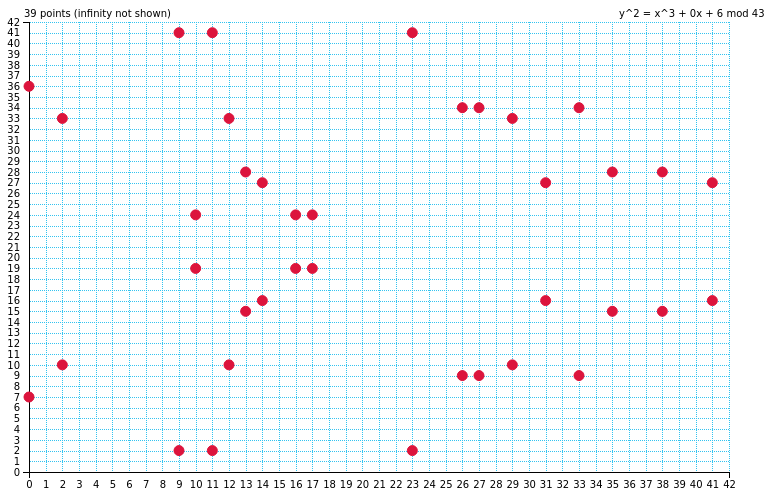
\includegraphics[scale=0.6]{/home/mirco/work/mmm/moonmath-manual/figures/bls6-6.png}
As we can see our curve is somewhat nice, as it does not contain self inverse points that is points with $y=0$. It follows that the addition law can be optimized, since the branch for those cases can be eliminated. 

Note: Is there a way to printe the entire addition table from https://graui.de/code/elliptic2/ here? Would be nice to have but is a bit large.

Since the order of BLS6-6 is $39= 3\cdot 13$, we know that it has a "large" subgroup of order $13$ and small subgroup of order $3$. We can use XXX to find those groups. We have $BLS6-6(3)=\{\mathcal{O},(0,7),(0,36)\}$.

In addition we have the generator $g_{BLS6}:=(13,15)$ that generates
\begin{multline}
BLS6-6(13)=\\
\{(13,15) \rightarrow (33,34) \rightarrow  (38,15) \rightarrow  (35,28) \rightarrow (26,34) \rightarrow  (27,34) \rightarrow  \\ 
(27,9)  \rightarrow  (26,9) \rightarrow  (35,15) \rightarrow  (38,28) \rightarrow  (33,9) \rightarrow (13,28) \rightarrow  \mathcal{O}\}$$
\end{multline}

Computations "in the exponent": In cryptography and in particular in snarks a lot HAPPENS IN THE EXPONENT...

To use our example to explain what this means observe that from this representation, we can deduce a map from the scalar field $\F_{13}$ to $BLS6-6(13)$ with respect to our generator. WE have
$$
[\cdot]_{(13,15)}: \F_{13} \to BLS6-6(13)\;;\; x \mapsto [x](13,15)
$$

So for example we have $[1]_{(13,15)}= (13,15)$, $[7]_{(13,15)}= (27,9)$ and $[0]_{(13,15)}= \mathcal{O}$. In particular this map is a homomorphism of groups from the additive group $\F_{13}$ to $BLS6-6(13)$. This means in particular, the the additive neutral element from $\F_{13}$ is mapped to $\mathcal{O}$ and negatives are mapped to inverses. For example $[-2]_{(13,15)}= - [2]_{(13,15)}$, since
$[-2]_{(13,15)}= [11]_{(13,15)}= (33,9) = (33,-34) = -(33,34)=
- [2]_{(13,15)}$

The map also give a visualization of the ECDL problem in $BLS6-6(13)$, which is concerned with finding solutions $x\in \F_{13}$ for the equation 
$[x]_{(13,15)}= (x,y)$ for any $(x,y) \in BLS6-6(13)$. Of course ECDL is not hard in $BLS6-6(13)$, since we can deduce the solutions easily from XXX. For example the solution to $[x]_{(13,15)}= (35,15)$ is $x=9$, since $[9](13,15)=(35,15)$.

Since $[0]_{(13,15)}$ maps the group of cyclic integers modulo $13$ onto our group $BLS6-6(13)$, we can use this to write down the group law in the following way:
\begingroup
    \fontsize{5pt}{5pt}\selectfont
$$
\begin{array}{c|ccccccccccccc}
\cdot & \mathcal{O}  & (13,15) & (33,34) & (38,15) & (35,28) & (26,34) & (27,34) & (27,9) & (26,9) & (35,15) & (38,28) & (33,9) & (13,28)\\
\hline
\\
\mathcal{O} & \mathcal{O}  & (13,15) & (33,34) & (38,15) & (35,28) & (26,34) & (27,34) & (27,9) & (26,9) & (35,15) & (38,28) & (33,9) & (13,28)\\
\\
(13,15) & (13,15) & (33,34) & (38,15) & (35,28) & (26,34) & (27,34) & (27,9) & (26,9) & (35,15) & (38,28) & (33,9) & (13,28) & \mathcal{O}\\
\\
(33,34) & (33,34) & (38,15) & (35,28) & (26,34) & (27,34) & (27,9) & (26,9) & (35,15) & (38,28) & (33,9) & (13,28) & \mathcal{O} & (13,15)\\
\\
(38,15) & (38,15) & (35,28) & (26,34) & (27,34) & (27,9) & (26,9) & (35,15) & (38,28) & (33,9) & (13,28) & \mathcal{O} & (13,15) & (33,34)\\
\\
(35,28) & (35,28) & (26,34) & (27,34) & (27,9) & (26,9) & (35,15) & (38,28) & (33,9) & (13,28) & \mathcal{O} & (13,15) & (33,34) & (38,15)\\
\\
(26,34) & (26,34) & (27,34) & (27,9) & (26,9) & (35,15) & (38,28) & (33,9) & (13,28) & \mathcal{O} & (13,15) & (33,34) & (38,15) & (35,28)\\
\\
(27,34) & (27,34) & (27,9) & (26,9) & (35,15) & (38,28) & (33,9) & (13,28) & \mathcal{O} & (13,15) & (33,34) & (38,15) & (35,28) & (26,34)\\
\\
(27,9) & (27,9) & (26,9) & (35,15) & (38,28) & (33,9) & (13,28) & \mathcal{O} & (13,15) & (33,34) & (38,15) & (35,28) & (26,34) & (27,34)\\
\\
(26,9) & (26,9) & (35,15) & (38,28) & (33,9) & (13,28) & \mathcal{O} & (13,15) & (33,34) & (38,15) & (35,28) & (26,34) & (27,34) & (27,9)\\
\\
(35,15) & (35,15) & (38,28) & (33,9) & (13,28) & \mathcal{O} & (13,15) & (33,34) & (38,15) & (35,28) & (26,34) & (27,34) & (27,9) & (26,9)\\
\\
(38,28) & (38,28) & (33,9) & (13,28) & \mathcal{O} & (13,15) & (33,34) & (38,15) & (35,28) & (26,34) & (27,34) & (27,9) & (26,9) & (35,15)\\
\\
(33,9) & (33,9) & (13,28) & \mathcal{O} & (13,15) & (33,34) & (38,15) & (35,28) & (26,34) & (27,34) & (27,9) & (26,9) & (35,15) & (38,28)\\
\\
(13,28) & (13,28) & \mathcal{O} & (13,15) & (33,34) & (38,15) & (35,28) & (26,34) & (27,34) & (27,9) & (26,9) & (35,15) & (38,28) & (33,9)\\
\end{array}
$$
\endgroup


Cofactor clearing: 

Given an arbitrary point on the curve that is not in any of our two subgroups like $(2,33)$, we can project it on both subgroups $BLS6-6(3)$ and $BLS6-6(13)$ respectively, by \textit{multiplication with the cofactor}. Since $39 = 3 \cdot 13$, we have to multiply $(2,33)$ with $13$ to map it onto $BLS6-6(3)$ and we have to multiply $(2,33)$ with $3$ to map it onto $BLS6-6(13)$. Indeed we get $[13](2,33)= (0,36)$ which is an element of $BLS6-6(3)$ and $[3](2,33)= (35,15)$ which is an element of $BLS6-6(13)$
\paragraph{MNT-Curve Cycles}
